\chapter{Protocolli di QKD}
\label{chap:protocolli_qkd}
Diversamente da molti dei protocolli crittografici classici oggi in uso, la cui sicurezza si basa spesso su ipotesi non dimostrate riguardanti la complessità computazionale di problemi matematici, la sicurezza della crittografia quantistica si basa sulle leggi della fisica. Su tali leggi i protocolli di QKD, che rappresentano una porzione corposa della crittografia quantistica, basano la propria sicurezza incondizionata.\\

In questo capitolo verranno descritti i funzionamenti dei protocolli di QKD BB84, B92, E91 e SARG04. Alcuni di questi si basano sul principio di indeterminazione di Heisenberg, mentre altri sul principio di Entanglement. Tali protocolli, selezionati fra tutti perché rappresentano le basi di numerosi protocolli di QKD più recenti, verranno presentati in ordine cronologico di pubblicazione.\\

\section{BB84}
Il protocollo BB84 \cite{bb84}, ideato a C. H. Bennet e G. Brassard nel 1984, è un protocollo di QKD basato sul principio di indeterminazione di Heisenberg che sfrutta gli stati di polarizzazione dei fotoni per trasmettere l'informazione.\\
Il mittente e il ricevente (Alice e Bob) sono intenzionati a scambiarsi una chiave segreta e sono connessi l'una all'altro mediante un canale quantistico, su cui viaggiano i fotoni polarizzati, e un canale classico di comunicazione (ad esempio Internet). Nessuno dei due canali ha la necessità di essere sicuro, dal momento che BB84 è progettato ipotizzando la presenza di un \textit{eavesdropper} (Eve) che può interferire nelle comunicazioni su ambo i canali. Come indicato nel capitolo \ref{chap:background}, il canale quantistico può essere manomesso ma non monitorato passivamente; per il canale classico, invece, valgono le considerazioni inverse.\\
Le polarizzazioni dei fotoni, o stati, sono quattro e sono raggruppate in due diverse basi non ortogonali: quella rettilinea ($\bigoplus$) e quella diagonale ($\bigotimes$). La base $\bigoplus = \{\ket{0}, \ket{1}\}$ , mentre la base $\bigotimes = \{\ket{+}, \ket{-}\}$, dove $\ket{+} = \frac{1}{\sqrt{2}}(\ket{0}+\ket{1})$ e $\ket{-} = \frac{1}{\sqrt{2}}(\ket{0}-\ket{1})$. La figura \ref{fig:non_orthogonal_bases} riporta i 4 possibili stati quantistici previsti da BB84 raggruppandoli per base di polarizzazione: BB84 assegna allo stato $\ket{0}$ e $\ket{+}$ la codifica dello 0 binario, mentre a $\ket{1}$ e $\ket{-}$ la codifica del 1 binario.

\begin{figure}[h]
    \centering
    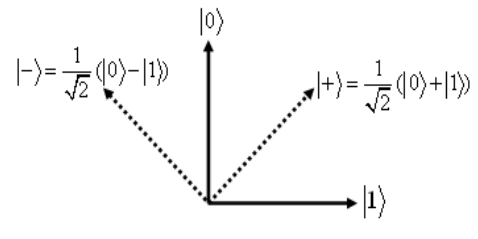
\includegraphics[width=10cm]{immagini/non_orthogonal_bases.png}
    \caption{I quattro diversi stati di polarizzazione dei fotoni nel protocollo BB84 \cite{elboukhari}}
    \label{fig:non_orthogonal_bases}
\end{figure}

Di seguito sono indicati i passi del protocollo come riassunti da \cite{elboukhari}:
\begin{enumerate}
    \item Alice costruisce una stringa casuale di bit $s \in \{0,1\}^n$ e una stringa casuale di basi $b \in \{\bigoplus, \bigotimes\}^n$ per la codifica;
    \item Alice prepara $n$ qubit $q_i$ polarizzando altrettanti fotoni usando la base $b_i \in b$ per la codifica del bit $s_i \in s$;
    \item Alice spedisce i qubit a Bob su un canale quantistico pubblico;
    \item Bob costruisce una stringa casuale $b' \in \{\bigoplus, \bigotimes\}^n$ di basi che verranno utilizzate per la misurazione degli $n$ qubit inviati da Alice. Misurandoli, ottiene una stringa di bit $s' \in \{0,1\}^n$;
    \item per ogni bit $s_i \in s$, Alice invia a Bob su un canale classico il valore di $b_i$ e Bob verifica se $b_i = b'_i$. In caso negativo, i bit $s_i$ e $s'_i$ vengono rimossi rispettivamente da $s$ e da $s'$;
    \item Alice quindi individua un sottoinsieme casuale di bit in $s$ e li comunica a Bob sul canale classico. Se anche solo uno di questi bit non coincide con la misurazione effettuata da Bob sul qubit corrispondente, allora viene rilevata la presenza di un \textit{eavesdropper} Eve sul canale quantistico e cessano le comunicazioni tra Alice e Bob;
    \item se invece tutti i confronti danno esito positivo, allora i bit rimasti in $s$ compongono la chiave segreta $ k = \{0,1\}^t$, con $t < n$.
\end{enumerate}

Per capire correttamente il funzionamento di BB84 occorre spiegare come avviene la misurazione di un qubit secondo una qualche base. Se si ha $\ket{qubit} = a\ket{c} + b\ket{d}$ la misura di questo stato utilizzando la base $B = \{\ket{c}, \ket{d}\}$ produce lo stato $\ket{c}$ con probabilità $|a|^2$  e lo stato $\ket{d}$ con probabilità $|b|^2$. Ovviamente i quadrati delle ampiezze di a e b se sommati restituiscono 1. Quindi, se misurassimo lo stato $\ket{qubit}$ con una base diversa, il risultato ottenuto sarebbe casuale. Nel caso di Bob, se sceglie di utilizzare la base $\bigotimes$ per misurare un qubit in stato $\ket{1}$, il risultato della misurazione sarà equiprobabilmente 0 oppure 1. Al contrario, se sceglie di utilizzare la base $\bigoplus$ allora otterrà certamente 1 dal momento che $\ket{1} = 1\ket{1}+0\ket{0}$.\\

I test condotti durante il passo 6 sono pensati precisamente per rilevare la presenza di Eve. Se uno di essi fallisce, il motivo può essere un disturbo esterno oppure un rumore sul canale quantistico, ma si suppone in entrambi i casi che la causa sia la presenza di Eve. Infatti, tra gli attacchi che può effettuare, c'è anche il cosiddetto \textit{intercept-resend}, dove Eve misura lo stato dei fotoni inviati da Alice e poi invia a Bob nuovi fotoni polarizzati in base allo stato che lei stessa ha misurato. Dal momento che Eve non ha idea delle basi che Alice ha utilizzato per la polarizzazione dei fotoni, può solamente provare ad indovinarle proprio come fa Bob. Se Eve sceglie la base corretta, allora misura il corretto stato di polarizzazione e rinvia a Bob lo stato corretto. Tuttavia, se la base che sceglie non è corretta, allora lo stato che viene misurato è casuale così come lo stato del qubit che verrà rinviato a Bob. In quest'ultimo caso, il principio di indeterminazione garantisce che l'informazione codificata in tale qubit venga persa. Giunti a questo punto, se la misurazione dello stato effettuata da Bob sfrutta la stessa base utilizzata da Alice, allora lo stato misurato sarà casuale. \\

Eve sceglie le proprie basi erroneamente con una probabilità di 0.5 per ciascuna e, se Bob misura i fotoni precedentemente intercettati da Eve utilizzando le stesse basi di Alice, allora anche lui ottiene un risultato sbagliato con una probabilità di 0.5. Quindi, la probabilità che un qubit intercettato generi un bit errato nella chiave finale è di $0.5 * 0.5 = 0.25$. Se poi Alice e Bob confrontano pubblicamente $n$ bit della loro chiave, allora la probabilità di ottenere un confronto dall'esito negativo e di rilevare la presenza di Eve è pari a $1 - (\frac{3}{4})^n$. Quindi, maggiore è il numero dei bit della chiave e maggiore sarà la probabilità di rilevare l'eventuale presenza di un \textit{eavesdropper} \cite{elboukhari}. \\

BB84 a oggi è il protocollo di QKD più famoso e il più implementato. La sua capacità di rilevare la presenza di \textit{eavesdropper} è stata provata in \cite{mayers} e \cite{shor_preskill}. Il canale quantistico maggiormente utilizzato è la fibra ottica \cite{hughes}, anche se è possibile utilizzare elettroni e quindi canali di trasmissione basati su conduttori elettrici o spazio libero \cite{knight}.

\section{E91}
Il protocollo E91 \cite{e91}, che prende il nome dal suo ideatore (A. Ekert) e dall'anno in cui è stato pubblicato, si basa sul principio di Entanglement e sfrutta coppie di particelle, dette EPR (Einstein-Podolsky-Rosen), correlate dal punto di vista quantistico. Queste coppie di stati quantistici costituiscono quegli stati, mostrati di seguito, su cui si basa E91.

\begin{enumerate}
    \item $\ket{S_0} = \frac{1}{\sqrt{2}}(\ket{00}+\ket{11})$
    \item $\ket{S_1} = \frac{1}{\sqrt{2}}(\ket{00}-\ket{11})$
    \item $\ket{S_2} = \frac{1}{\sqrt{2}}(\ket{10}+\ket{01})$
    \item $\ket{S_3} = \frac{1}{\sqrt{2}}(\ket{10}-\ket{01})$
\end{enumerate}

Il funzionamento del protocollo \cite{e91} viene indicato di seguito:
\begin{enumerate}
    \item Alice crea una sequenza di $n$ coppie EPR, cioè di fotoni polarizzati e quantisticamente correlati. Per ogni coppia, invia un fotone a Bob e memorizza l'altro in una memoria quantistica;
    \item Sia Alice che Bob scelgono casualmente una sequenza di $n$ basi  ($\bigoplus$ o $\bigotimes$). Tali basi saranno utilizzate sia da Alice che da Bob per misurare i fotoni della sequenza: quelli memorizzati da Alice e quelli ricevuti da Bob;
    \item Alice e Bob comunicano su un canale classico le proprie misurazioni e conservano unicamente quelle che sono state ottenute utilizzando la stessa base. I bit conservati compongono una cosiddetta \textit{raw key}, mentre quelli scartati compongono una \textit{rejected key}.
    \item Alice e Bob confrontano le proprie \textit{rejected key} per verificare che la disuguaglianza di Bell sia o meno soddisfatta: in caso affermativo, viene rilevata la presenza di un \textit{eavesdropper} Eve perché normalmente la disuguaglianza non è valida per coppie EPR; in caso negativo, Eve non è presente.
\end{enumerate}

Dalla descrizione del funzionamento di E91 emerge quindi come anche questo protocollo sia concepito per rilevare la presenza di un \textit{eavesdropper}. Questa verifica però avviene in modo diverso rispetto agli atri protocolli trattati in questo documento: in questo caso, infatti, viene testata la disuguaglianza di Bell, invece che verificate le "incongruenze" fra bit. Semplicemente, la disuguaglianza di Bell verifica la correlazione quantistica tra particelle che compongono una coppia EPR. La misurazione di una di esse da parte di Eve "rompe" lo stato di Entanglement che esiste fra le due, portando la disuguaglianza di Bell ad essere valida quando normalmente non lo è. Questa verifica funge quindi da campanello di allarme per segnalare ad Alice e Bob la presenza di Eve.

I passi succitati descrivono il funzionamento del protocollo E91 nella sua versione originale. Tuttavia, negli anni, numerosi ricercatori hanno pubblicato leggere varianti del protocollo (\cite{hwang}, \cite{lomonaco}).

A oggi, esistono implementazioni simulate di E91 all'interno dell'ambiente Matlab \cite{matlab_impl}, ma sono state realizzate anche delle implementazioni reali, seppur sperimentali, tramite una rete satellitare \cite{ent_impl}. Infatti, l'impiego di un satellite nella composizione di canali quantistici risolve il problema del degrado del \textit{photon trasmission rate}, che affligge invece la fibra ottica quando questa supera una data lunghezza (dell'ordine di centinaia di chilometri).

\section{B92}
Il protocollo B92 \cite{b92}, nato nel 1992 ad opera di C. Bennet, si basa su due stati quantistici non ortogonali. B92 condivide lo stesso principio quantistico di funzionamento di BB84, ma utilizza solamente due stati quantistici invece che quattro.
Di seguito sono indicati i passi del protocollo come descritti da \cite{elboukhari}:
\begin{enumerate}
    \item  Alice sceglie casualmente gli elementi di un vettore $A \in \{0,1\}^n$. Per ogni $i=1,...,n$, se $A_i = 0$ Alice invia a Bob lo stato $\ket{0}$ sul canale quantistico, mentre se $A_i = 1$ allora Alice invia $\ket{+}$;
    \item Bob crea un proprio vettore di bit casuali detto $B \in \{0,1\}^n$. Per ogni $i=1,...,n$, se $B_i = 0$ Bob sceglie la base $\bigoplus$, mentre sceglie invece la base $\bigotimes$ se $B_i = 1$;
    \item con tali basi ($\bigoplus$ o $\bigotimes$), Bob misura ogni stato quantistico inviato da Alice ($\ket{0}$ o $\ket{+}$);
    \item Bob costruisce il vettore $T \in \{0, 1\}^n$ in questo modo: per ogni $i=1,...,n$, se la misura effettuata da Bob sul qubit $q_i$ inviato da Alice produce $\ket{0}$ o $\ket{+}$ allora $T_i = 0$; diversamente, se la misurazione effettuata da Bob produce $\ket{1}$ o $\ket{-}$, allora $T_i = 1$;
    \item Bob invia T ad Alice sul canale di comunicazione classico;
    \item Alice e Bob conservano solamente i bit di A e di B in corrispondenza di $T_i = 1$. In questo modo, e supponendo l'assenza di Eve, vale che $A_i = 1 - B_i$. I bit preservati compongono quindi una chiave grezza condivisa formati dagli $A_i = 1- B_i$;
    \item Alice sceglie un campione dei bit della chiave grezza condivisa e ne rivela i bit a Bob su un canale classico. Se esiste anche solo uno di essi per cui vale che $A_i \neq 1 - B_i$, allora viene rilevata la presenza di Eve e le comunicazioni fra Alice e Bob vengono interrotte.
    \item la chiave segreta condivisa $K \in \{0, 1\}^t$, con $ t < n$ è quindi costruita rimuovendo dalla chiave grezza i bit campionati al passo precedente.
\end{enumerate}

Per capire correttamente B92 occorre notare che se un $T_i = 0$ significa che Bob non sa cosa Alice gli abbia inviato. Quindi se Bob sceglie $\bigoplus$ ($\bigotimes$) come base, può ottenere $\ket{0}$ ($\ket{+}$) come risultato della propria misurazione qualunque sia lo stato realmente inviato da Alice ($\ket{0}$ oppure $\ket{+}$). Invece, se $T_i = 1$ allora Bob saprà con esattezza qual è lo stato che gli è stato inviato da Alice. Inoltre, al passo 6, Alice e Bob verificano l'eventuale presenza di Eve. L'idea è che se esiste un $i$ tale che $T_i = 1$, allora $A_i = 1 - B_i$; altrimenti, è evidente che esiste del rumore sul canale quantistico o che vi è stato applicato un disturbo esterno (entrambi i casi si suppone siano riconducibili alla presenza di Eve). La tabella in figura \ref{fig:tab_b92} riassume e chiarifica il funzionamento di B92.
\begin{figure}[h]
    \centering
    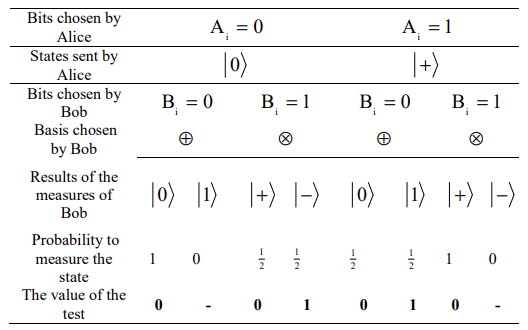
\includegraphics[width=10cm]{immagini/tab_b92.png}
    \caption{Descrizione riassuntiva del protocollo B92 \cite{elboukhari}}
    \label{fig:tab_b92}
\end{figure}\\
Anche questo protocollo è capace di rilevare la presenza di eventuali \textit{eavesdropper}. Le implementazioni, dal momento che si utilizzano ancora fotoni polarizzati per l'invio degli stati quantistici, coinvolgono ancora l'utilizzo di fibre ottiche come canali, sorgenti e ricettori di fotoni per l'invio e la ricezione degli stessi. Anche in questo caso, però, come per BB84, sono state realizzate implementazioni reali, seppur sperimentali, basate su elettroni polarizzati che viaggiano su conduttori elettrici o nello spazio libero \cite{knight} \cite{hughes}.

\section{SARG04}
\label{sec:sarg04}
Il protocollo SARG04 \cite{sarg04} è una variante di BB84 che si fonda quindi sul medesimo principio quantistico. La prima fase, quella che va dal passo 1 fino al passo 4 incluso, è pressoché identica. Una differenza sostanziale si nota nel passo 5, ossia quando Alice e Bob comunicano su un canale tradizionale per quali bit le basi che hanno utilizzato nelle misurazioni coincidono. In SARG04 Alice non annuncia direttamente a Bob le proprie basi, bensì gli invia una coppia di stati non ortogonali di cui uno è stato utilizzato per la codifica del bit corrispondente. In questo modo, se Bob ha scelto la base corretta, allora misurerà lo stato corretto e anche il bit originariamente inteso da Alice. Diversamente, non sarà in grado di misurare correttamente nessuno dei due stati non ortogonali inviati da Alice e non riuscirà a risalire al bit originale.
Un'altra differenza sostanziale sta nel fatto che SARG04 non utilizza una sorgente a singolo fotone come BB84 o B92, bensì un laser a impulsi attenuati. Questa differenza, a livello fisico invece che algoritmico, rende SARG04 più robusto di BB84 ad attacchi di tipo PNS \cite{elboukhari} dal momento che è più difficile prelevare un gran numero di fotoni che sono raggruppati in impulso luminoso senza rivelare la propria presenza.
Anche SARG04, in quanto derivato di BB84 rende possibile la rilevazione di eventuali \textit{eavesdropper}.